\documentclass[conference]{IEEEtran}
\IEEEoverridecommandlockouts
% The preceding line is only needed to identify funding in the first footnote. If that is unneeded, please comment it out.
\usepackage{cite}
\usepackage{amsmath,amssymb,amsfonts}
\usepackage{algorithmic}
\usepackage{graphicx}
\usepackage[inline]{enumitem}
\usepackage{textcomp}
\usepackage{xcolor}
\usepackage{csquotes}
\usepackage{fancyvrb}
\usepackage{verbatim}
\usepackage{url}

\newcommand\hl[1]{\colorbox{red!10}{#1}}
\newcommand{\ajay}[1]{{\color{magenta} {\bf Ajay:} #1}}

%%%%%%%%%% use lower capse for table caption
\usepackage{etoolbox}
\makeatletter
\patchcmd{\@makecaption}
  {\scshape}
  {}
  {}
  {}
\makeatother
%%%%%%%%%%%

\def\BibTeX{{\rm B\kern-.05em{\sc i\kern-.025em b}\kern-.08em
    T\kern-.1667em\lower.7ex\hbox{E}\kern-.125emX}}
    
    
\begin{document}

\title{A Benchmark Suite for Validating x86 Performance Model\\
}

%\author{\IEEEauthorblockN{1\textsuperscript{st} Given Name Surname}
%\IEEEauthorblockA{\textit{dept. name of organization (of Aff.)} \\
%\textit{name of organization (of Aff.)}\\
%City, Country \\
%email address}
%}

\maketitle

\begin{abstract}
%Modern microprocessors have undergone decades of hardware optimizations.
%For example, modern x86-64 microprocessors employ sophisticated
%instruction execution paths with heavily pipelined,
%out-of-order, super-scalar execution units that are highly complex.
%Producing code that
%exploits and optimizes for this underlying execution environment requires careful
%modelling of the microprocessor functionality. To achieve this, modern compilers employ processor models that predict
%the cost of
%executing a set of instructions to perform backend optimizations such as instruction
%selection, register allocation, instruction scheduling etc.
%\ajay{The lines till here sound a bit repetitive. We are not saying anything concrete here. All we are saying is microprocessors are complex}.
%\ajay{Also, mentioning x86\_64 as an example is a bit misleading. Because we do only for x86\_64. We should start directly with - Modern x86\_64 employs}.
%However, these cost models receive less attention than optimizations themselves.
Modern x86 processors have complex performance characteristics due
to micro-architectural optimizations such as \chcomment{pipelining, super-scalar,} out-of-order executions and micro-op fusions.
To reduce the complexity of optimizing for these processors,
many optimization techniques, manual or automatic, use cost models
to abstract away target machines.
Inaccurate models can cause misoptimizations.
There are known, sometimes significant issues of
cost models in production compilers such as LLVM\cite{llvm} and machine code analyzers
written by processor vendors themselves such as IACA\cite{iaca}.
IACA has been shown in some cases to deviate from the measured throughput
of a basic block of instructions by more than 2x.
Despite this, there is no standard, systematic approach or tooling
to perform validation and tuning of processor cost models.

In this paper, we present the necessary tooling and a benchmark suite
for validating and tuning cost models of x86-64 basic blocks.
Our benchmark suite contains more than 300,000 \chcomment{should have the number for the entire suite}
basic blocks extracted from a wide range of applications.
We describe our techniques to profile arbitrary basic blocks automatically and accurately;
which entails much more than simply measuring the latency of an unrolled basic blocks;
in fact our ablation study shows that the profiling \textit{without} some of our measures
ranges from crashing to obtaining results that are orders of magnitude away from the ground truth.\chcomment{
Something on how hard measurement is?}
We analyze the benchmark suite and show how and where popular
cost models used by static predictors such as llvm-mca, IACA, Ithemal and
OSACA\cite{osaca} deviate from the ground truth measured data.
We show that in certain classes of basic blocks
(e.g. vectorized numerical kernels) even the most accurate
model is on average more than 30\% away from the ground truth.
Furthermore, our dataset can be used as training data for learning-based cost models, such as in Ithemal.

%In addition to cost model validation,
%our dataset and the profiling infrastructure is useful
%for data-driven cost model construction\cite{ithemal}.

%In spite of this, compiler cost models undergo low levels
%of validation and scrutiny due to the lack of tolling and
%test suites that generate validation data.


% Modern super-scalar out-or-order processors are complex objects.
% To reduce the complexity of optimizing for these processors,
% many optimization techniques, manual or automatic, use cost models
% to abstract away target machines.
% Cost models however receive less attentions than optimizations,
% and inaccurate models can cause miss optimizations.
% There are known, sometimes significant issues of
% cost models in production compilers such as LLVM\cite{llvm,goslp}.
% Even IACA, Intel's own throughput predictor has
% been shown in some cases to deviate from measured throughput
% by more than 100\%.

% Despite the importance of existing cost models,
% to this day there is no standard, systematic approach 
% to perform cost model validation and tuning.
% We describe a benchmark for validating performance 
% models of x86 basic blocks.
% Our dataset contains more than three hundred thousand
% basic blocks extracted from a wide range of applications.
% We describe our technique to profile the throughput
% of these basic blocks automatically and accurately.
% We automatically classified our basic blocks by their use
% of CPU resources and evaluated accuracy of existing cost models
% for different classes of basic blocks. 
% We showed that in certain classes of basic blocks 
% (e.g. vectorized numerical kernels) even the most accurate
% model is on average more than 30\% away from the ground truth.
% In addition to cost model validation,
% our dataset and the profiling infrastructure is useful
% for data-driven cost model construction\cite{ithemal}.
\end{abstract}
\begin{IEEEkeywords}
performance models, basic block profiler, x86-64, basic block benchmark suite
\end{IEEEkeywords}
\section{Introduction}
Many optimizations, whether manual or automatic,
benefit from performance models.
Static performance models such as IACA lessen programmers
the burden of isolating performance kernels from
the rest of the applications,
and of properly implementing micro-benchmark. Many compiler optimizations
use cost models of one form or another:
a typical automatic vectorizer, for instance,
use one to estimate the cost of vector packing
in the presence of irregular memory accesses~\cite{goslp};
instruction schedulers uses one to model the latency
and throughput of instructions~\cite{llvm-sched,gcc-sched}.

Cost models however often take a back seat to “actual” optimizations,
despite the accuracy of former ensures the effectiveness of latter.
For instance, Mendis et al.\cite{goslp}
recently published a technique to perform optimal\footnote{
Witch certain caveat.
In particular their formulation is optimal
only when the target machine only has vector-width of 2}
SLP Vectorization\cite{slp} that
incurred slowdown in some instances due to the inaccuracy of 
LLVM's cost models.
Without a comprehensive benchmark to pinpoint the weakness of their models,
developers cannot systematically improve these cost models;
model parameters
such as the throughput of individual instructions
are sometimes chosen haphazardly;
consider following quote taken from a commit message from LLVM\cite{llvm}
regarding its cost model\footnote{
https://reviews.llvm.org/D46276.
}:
\begin{quote}
X86's fix to avoid SDIV/UDIV vectorization is clumsy
(multiplying the vector costs x20)
and appears to have been implemented before the cost of
scalarization was being realistically accounted for...
\end{quote}

We describe a benchmark for validating performance models
of x86 basic blocks.
In this work we focus on throughput prediction.
We make the following contributions:
\begin{enumerate}
\item We collected basic blocks from a wide range of domains.
This data set, together with additional profile information we collected,
can be used to design and validate low level optimizations
such as backend peephole optimizers,
in addition to its primary purpose of model validation.

\item We describe a fully automatic technique
for measuring the throughput of basic blocks extracted 
from raw binaries.
This is much more than simply measuring the latency of an unrolled basic block
since code snippets with memory accesses (and most do)
generally cannot be executed safely
outside of the context of their source applications.
We have used this technique to profile the throughput of more than 2 million basic blocks.
Our methodology, when implemented, is accurate and fast.
Depends on the context -- 
if a developer is only interested in the performance of a code snippet
but not how constituent instructions contribute to the final
throughput -- our tool outperforms IACA in both speed and accuracy.

\item We automatically classified the basic blocks
by their usage of different execution ports.
This classification allows developers to pinpoint weakness
of their performance models.
Maintainers of an automatic vectorizer, for instance,
can use this to fine-tune cost models
of vectorized basic blocks.

\item We evaluated four existing cost models:
IACA, llvm-mca -- 
which exposes LLVM’s internal optimization cost models,
OSACA\cite{osaca}, and Ithemal\cite{ithemal}.
We breakdown the strength and weakness of these cost models on
different classes of basic blocks;
e.g. we show that all such tools
have average error higher than 30\% 
when used to analyze numerical kernels running on Haswell machines.



\end{enumerate}
\section{Background}

\subsection{Existing Performance Models}
\label{sec:perf-models}

IACA~\cite{iaca} (Intel Architecture Code Analyzer) is a static analyzer
developed by Intel. It has support for Intel micro-architectures
since Nehalem.
Given a machine code snippet, IACA estimates the average number
of cycles it costs to execute the given code in an infinite 
loop.
Unlike its alternatives, IACA takes advantage of its knowledge
of Intel's proprietary processor optimization---such as zero-idioms and micro-op fusions---to make better 
predictions.

llvm-mca~\cite{llvm-mca} is a similar tool inspired by IACA. 
Implemented as an out-of-order super-scalar simulator,
it uses parameters (e.g., instruction throughput)
supplied by LLVM\cite{llvm}'s backend scheduling model.
Reusing of the scheduling model is an explicit design choice
made to expose LLVM's cost model for testing.
Thus the accuracy of llvm-mca has a bearing on
that of LLVM's scheduling model.

OSACA\cite{osaca} is an analyzer developed as the open-source
alternative to IACA. It is similar to llvm-mca in that
it is implemented as a parametrized out-of-order simulator---in
this case, the parameters come from the measured throughput
and latency data for individual instructions.

Ithemal\cite{ithemal} is a basic block throughput predictor
implemented as a deep neural network. Unlike other models discussed so far, 
tools, Ithemal is not a simulator in the sense that it outputs
a single throughput prediction for each input basic block
without reporting an interpretable execution trace.

Production compilers such as LLVM\cite{llvm} and GCC typically use cost models 
to guide optimizations.
Unlike ``user-facing'' models such as IACA or llvm-mca, these cost models typically
model the costs at the instruction level, rather than at whole basic block level.
These compilers also use multiple cost models.
LLVM, for instance uses (at least) three cost models: 
a generic, per-instruction IR cost model in its middle-end IR~\cite{llvm-cost};
one that captures the information required for instruction scheduling,
(i.e. the scheduling model~\cite{llvm-sched}, also used by llvm-mca);
and another one that models the cost of register uses---such as cost of loads
and register-to-register transfer---in register allocation~\cite{llvm-reg}.
GCC similarly employs analogous models~\cite{gcc-cost,gcc-sched}.
Out of the models discussed so far, to our best knowledge, 
the scheduling model of LLVM is the only one exposed by an interface
(in this case, llvm-mca) for testing in isolation from its client optimizations.
% TODO: can we make a stronger statement saying given our work, we think
% other models should be exposed as well?


\vspace{1em}
\noindent{\bf Modeling Assumptions.}
All of cost models discussed above make the following assumptions about the execution context
of the code they are modeling
\begin{itemize}
    \item All memory accesses hit the L1-cache.
    \item All instructions reside in the instruction cache.
    \item The execution is unaffected by context switches and interrupts.
\end{itemize}

\subsection{Existing Validation Tools and Profilers}
We briefly discuss existing tools and sources used by developers to validate
processor performance  models.
There are roughly two categories of these sources:
\begin{enumerate*}
\item per-instruction cost table tabulated either by
consulting the manual or manual benchmarking;
\item machine code profiler for running microbenchmarks.
\end{enumerate*}

\textbf{Per-instruction Latency/Throughput Tables}
These datasets are created either by scraping hardware manual or
by manual profiling 
(to obtain the real instruction latency or throughput).
Current sources of per-instruction information are incomplete and sometimes inaccurate~\cite{uops}. 
More importantly, they do not lead directly to validating performance model at basic block level or more.
Although in general, it is possible to estimate the throughput of 
a basic block by inferring the scheduling of its instructions based on their
port usage---this is the approach taken by llvm-mca~\cite{llvm-mca} and OSACA\cite{osaca}---this
it is incomplete and does not take microarchitectural
optimizations that could alter the ``normal'' execution paths into account. 
Examples of these optimizations include micro-op fusion and zero-idioms.
Therefore, IACA\cite{iaca} is generally recognized as the more accurate analyzer
compared to its alternatives since it can exploit
private optimizations employed by Intel's processors.

Intel's manual\cite{intel-manual} provides the throughput and latency
of frequently used instructions.
Agner Fog\cite{agner} similarly provides a table of instruction throughput and latency.
Google's EXEgesis team~\cite{exegesis} provides a tool that can automatically extract
machine-readable instruction specifications from Intel's manual.
llvm-exegesis, designed by the same team, is a tool that determines
the latency of an input instruction opcode\footnote{
Currently the tool is limited to instructions that does not touch memory or floating point registers} 
by automatically generating a micro-benchmark that measures the opcode's average latency;
some LLVM's developers use the tool to validate LLVM's scheduling model.

Abel and Reineke\cite{uops} recently published their methodology
to reverse engineer the detailed mapping from each instruction to the
combination of execution ports
that these micro-ops can use.
They build instruction-to-port mapping using automatically generated micro-benchmarks.
Based on this mapping, they infer the steady-state scheduling of constituent
micro-ops for an instruction and calculate the instruction throughput based on
this inferred schedule.

\textbf{Machine Code Profiler} These tools allow users to perform
detailed microbenchmarking and are used by compiler writers manually
to verify compiler cost models.
These profilers are, however, unsuitable for our work---i.e., profiling
a large set of arbitrary basic blocks for systematic validation.
They require user intervention to profile arbitrary basic blocks. Most notably,
user annotation is needed to allocate memory and
initialize memory-addressing registers to prevent crashing.

Agner Fog~\cite{agner} provides a script to profile small code snippets.
The script reports the number of cycles as well as performance statistics such as 
the number of cache misses.
The script assumes that it is the user's responsibility to ensure
the successful execution of the benchmark;
for instance, the user is expected to allocate memory and initialize pointers.

nanoBench~\cite{nanobench} is a profiler similar to that of Agner Fog's~\cite{agner},
with two notable improvements.
It allows the user to specify which processor-specific hardware
to measure---in addition to cycle-counter. It also supports profiling in kernel-mode,
removing potential noise due to context-switches and interrupts.

% TODO:
% 1. talk about compiler cost models (both LLVM and GCC), mention that there is a chicken and egg issues
% 2. talk about stuff like agner fog's script
\section{Methodology}
%DESCRIBE HOW WE GATHER AND TIME BASIC BLOCKS 
\subsection{Basic Block Collection}
We selected the source applications of our basic blocks with two goals:
\begin{enumerate*}
    \item The set of applications should cover a diverse range
of domains to represent real world workload
    \item Their basic blocks should reflect input that concerns typical users of a performance model;
    compiler developers deals with
    basic blocks from general purpose programs,
    which have different characteristics
    than those from 
    high performance kernels. 
\end{enumerate*}

We selected Clang/LLVM\cite{llvm} (compiler),
Redis (in-memory database), SQLite (database), and Gzip (compression)
to collect basic blocks that represent
applications that are written in general purpose languages
like C and C++.
Basic blocks from these programs
typically have high memory traffic, and are usually not-vectorized.
We chose these applications because they are some of the mostly used
applications today; they are well tuned for performance;
and they all have sophisticated use of algorithms and data structures,
giving us a large source of diverse basic blocks.

We selected high performance kernels from the following domains:
cryptography (OpenSSL), scientific computing (OpenBLAS),
machine learning (TensorFlow\cite{tensorflow}),
and rendering/multimedia (Embree\cite{embree} and FFmpeg).
All aforementioned applications --
with the exception of TensorFlow and Embree -- 
have kernels written in assembly.
Embree is written in ispc\cite{ispc}, a data parallel language
designed specifically to target Intel's vector extensions.

We collected basic blocks from these applications using
a dynamic analysis implemented in DynamoRIO\cite{dynamorio},
which provides an API to record every basic block
executed at runtime.
We opted for dynamic analysis rather than static disassembly
because precise static disassembly of x86 binary
is undecidable.
We use the official benchmark suites of these applications\footnote{
Except for FFmpeg and Gzip, which to the best of our knowledge do not have
official benchmarks. For these two applications we use inputs
from https://openbenchmarking.org.
} to simulate realistic execution of these applications when performing
the dynamic analysis.

\subsection{Timing Infrastructure}
We now describe our approach to profiling basic block thoughput.
We use IACA's definition of throughput, i.e. 
the average number of cycles required to execute a basic block inside
an infinite loop.
We guarantee the following invariants for our measurements.
\begin{itemize}
\item All memory data reside in L1 cache.
This is what tools like llvm-mca and IACA assume.

\item Measurements should be free of interrupts, context switches,
and hyper-threading.
\end{itemize}

\textbf{Deriving throughput from latency}.
The basic strategy one usually takes to measure basic block throughput
is unrolling a basic block multiple times and divide the latency of the
unrolled basic block by the unroll factor.
Compared to running the basic block inside a loop,
unrolling has an advantage in that the measurement is not polluted by
the overhead incurred by looping.
A typical unroll factor is 100\cite{ithemal,uops}.
Such a high unroll factor can however incur significant
L1-icache misses for large basic blocks
(e.g. already unrolled inner-loop body of a GEMM kernel).
The issue with unrolling naively is that,
an unroll-factor small enough to fit the 
unrolled basic block into instruction cache is on the other hand
insufficient to hide the latency of the first few iterations.
We thus adopted a different strategy to cope with large basic blocks.

We unroll each basic block with two different unroll factors.
These factors should be large enough 
to warm-up the processor into steady state.
We then measure the latency of the two unrolled basic blocks,
calculate the difference in latency, and divide it 
by difference of the unroll factors.
The resulting number is the throughput of the basic block.
Consider a processor that enters steady state
after executing a basic block 10 iterations.
We measure the latency of this basic block expanded with
two unroll factors -- 10 and 20.
Suppose the resulting latency is 120 and 200 respectively,
we can then determine that the throughput of this basic block
is $\frac{200-120}{20-10} = 8$ cycles per iteration.

\textbf{Handling memory accesses}.
Consider the basic block in figure \ref{fig:mem-ex},
which is used to compute the CRC code of input bytes in Gzip.
Highlighted instructions shows flow of pointer values;
essentially \textit{bits} of \verb|rdx| are used to index into a lookup table, 
and the content of which is then used in the next iteration to 
update \verb|rdx|.
How would one profile the throughput of this basic block?
Without the original application context,
this basic block \textit{cannot} be directly executed.
Developer of Gzip familiar with this piece of code could 
setup a micro-benchmark properly by reproducing the
relevant lookup table used by this code snippet,
but such approach would not scale to the hundred of 
thousands of basic blocks in our data set, most of which contain memory accesses.
We needed some way to automatically generate the benchmarking environment
without apriori knowledge/assumption of the code being profiled.

\begin{figure}[h]
\begin{Verbatim}[commandchars=\#\{\}]
    add rdi, 1
    #hl{mov eax, edx}
    shr rdx, 8
    #hl{xor al, [rdi - 1]}
    movzx eax, al
    #hl{xor rdx, [8*rax + 0x4110ah0]}
    cmp rdi, rcx
\end{Verbatim}
\caption{Inner loop body of updcrc from Gzip.
This basic block cannot be directly executed because
of its memory accesses.}
\label{fig:mem-ex}
\end{figure}
%TODO: point out concretely why previous approach, including prefixing
% addresses with the array does not work

A possible solution\cite{ithemal} is rewriting
the basic block so that all memory accesses are
relative to a pre-allocated array.
For instance, \verb|mov [rdx], 1| is rewritten to
\verb|mov [addr_of_arr+rdx], 1|. 
This approach has several issues.
\begin{itemize}
    \item Executing some basic blocks back to back can result in a 
    diverging (e.g. strided) access pattern. 
    One would need to pre-allocate an unrealistically large array
    in order to  accommodate for this pattern, 
    Even when a sufficiently large buffer could be allocated,
    this access pattern can result in cache misses, 
    which we want to avoid.
    \item The rewriting scheme does not take stack accesses
    into account.
    \item Rewritten instructions can
    have larger encoding, which can affect throughput
    of front-end bound basic blocks.
\end{itemize}

We avoid these pitfalls with a new technique
that divides the profiling process into two stages:
\begin{enumerate*}
\item We profile the virtual pages accessed by
the basic block (were it to run without crashing)
and map those pages to a single physical page.
\item After the appropriate mappings are created,
the unrolled basic block is then executed normally under
the new page mapping.
\end{enumerate*}

\textbf{Page Mapping}. 
In addition to legalizing all memory accesses made by the basic block,
the mapping stage also ensures that all memory accesses stay in
the L1 cache.
Mapping is done by executing the unrolled basic block in a forked process
 monitored by a parent process using \verb|ptrace|.
Each attempt to access an unmapped virtual page is intercepted by
the monitoring process, which then instructs the 
executing process to create the appropriate mapping
and to restart execution from the \textit{beginning}
with all registers, memory values,
as well as flag registers reinitialized.
Re-initialization is done to ensure that in the final measurement
stage the trace of memory addresses computed by the 
unrolled basic block is \textit{identical} to that from the mapping stage.

We make additional optimizations to further
increase our chance of successfully obtaining clean measurements.
Prior to the mapping-run,
we unmap all pages (except those containing the basic block).
This allows us to run basic blocks that inadvertently
writes to library code such as libc.
The physical page is
always initialized to be filled with a “moderately sized” constant
(we used \verb|0x12345600| in our experiments)
to accommodate for indirect memory accesses.
To see why this is necessary,
consider a basic block that first loads a pointer $p$ from memory
and then de-references $p$.
If the value of $p$ is too low (e.g. 0)
or too high
(i.e. bigger than the maximum memory that
a user space program is allowed to addressed),
then we will not be able to map the virtual page pointed by $p$.

\textbf{Handling Subnormal Numbers}.
General speaking -- aside from division
and specialized instructions such as \verb|sqrt|
-- floating point instructions have constant timing
except when input of the operations are subnormal numbers.
In our experiments where we encountered subnormal numbers,
floating point operations can be slowed down by up to 20x.
To ``normalize'' our timing, we configured \verb|MXCSR| register
to disable gradual underflow.

\textbf{Avoiding context switches and interrupts}.
The execution phase of profiling is done in kernel mode
to avoid performance fluctuation incurred by context switches
and interrupts.
This is implemented as a kernel driver that executes
user-supplied function pointer in kernel mode.
Preemptions and interrupts are disabled during measurement.

One might ask, were all the precautions we took in profiling necessary?
Table \ref{tab:ablation} shows the effect of incrementally applying
different optimizations to remove measurement noise.
Without some of our optimizations, the measurement could be 
two orders of magnitude off in the worst case.

\begin{table}
\begin{tabular}{
|p{0.2\columnwidth}|p{0.18\columnwidth}|p{0.18\columnwidth}|p{0.18\columnwidth}|}
\hline (Additional) Optimizations &
Measured Throughput &
L1 D-Cache Misses &
L1 I-Cache Misses \\

\hline
None & Crashed & N/A & N/A \\

\hline
Page mapping & 6377.0 & 956 & 0 \\

\hline
Single physical page & 2273.7 & 0 & 0 \\

\hline
Disabling gradual underflow & 65.0 & 0 & 35 \\

\hline
Using smaller unroll factor & 59.0 & 0 & 0\\

\hline
\end{tabular}
\\
\caption{Measured throughput for a sample basic block when
different measurement optimizations are incrementally applied.
The basic block is extracted from one of the critical 
inner loop body of TensorFlow\cite{tensorflow}'s CNN training benchmark.}
\label{tab:ablation}
\end{table}


\subsection{Basic Block Classifications}\label{classification}
Our benchmark reports the accuracy of a performance model in two modes:
\begin{enumerate*}
\item Weighted error for each application
\item Average prediction error of different classes of 
basic blocks (e.g. performance prediction
of basic blocks in numerical kernels vs.
cryptographic kernels).
\end{enumerate*}

\textbf{Per-application error}.
We collected program counter samples
in our dynamic analysis.
Using this information, we are able to weight each basic block by
the approximate frequency with which it is executed during runtime.
Weighting the basic blocks allows us to focus on basic blocks that have
non-negligible effects on performance.
Most basic blocks collected from TensorFlow\cite{tensorflow},
for instance, are from infrequently executed code 
such as the Python interpreter or glibc;
weighting these basic blocks allows a user of the benchmark
to see an evaluation the performance model relevant
to the application's expected runtime cost.

\textbf{Per-class error}. 
We automatically classify the basic blocks into
to different categories.
The high-level approach we took was to first,
\begin{enumerate*}
\item map each basic block to a vector representation
that reflects its usage of hardware resources,
\item and then cluster the basic blocks by their vector representations.
\end{enumerate*}

Using results from Abel and Reineke\cite{uops},
we compute a port-combination mapping for each instruction.
For instance,
the port-combination mapping for \verb|xor rax, rbx| in Haswell
is $\{ p0156 \rightarrow 1 \}$ (using Abel and Reineke's notation);
in other words, this instruction is implemented 
with a micro-op that can be executed at port-0, 5, and 6.
In Haswell, there are 13 such port combinations for all userland instructions.
Accordingly, we create a 13-element vector for each instruction such that
the $i'$th element denotes the number of micro-ops can be executed
on the $i'$th port-combination.
Similarly, we compute a 13-element vector for each basic block
in our dataset by summing over the port-combination vectors
of all instructions in the basic block and normalizing the vector by 
the total number of micro-ops.

After obtaining vector representation for the basic blocks, 
we used K-means\cite{kmeans} to partition the basic blocks into 20 clusters.
Table \ref{tab:clusters} gives a brief summary of the superficial characteristics
of each cluster; as the summary suggests, our clustering has semantic meaning.
We settled on using 20 clusters to balance
the tradeoff between the uniqueness of each cluster
and similarity of basic blocks within the same cluster;
using less clusters caused multiple partitions to have
near identical distributions of basic blocks,
and using too many grouped dissimilar basic blocks together.
Figure\ref{fig:apps_vs_clusters} shows the breakdown of each applications
by the classification of its basic blocks.
\begin{table}
\begin{tabular}{|p{0.15\columnwidth}|p{0.6\columnwidth}|p{0.1\columnwidth}|}
    \hline
    Cluster & Description & Size \\
    \hline
    
    Cluter-1 & 
    Loads mixed with few ALU ops & 49873 \\
    \hline
    
    Cluster-2 &
    Stores mixed with few ALU ops & 13062 \\
    \hline
    
    Cluster-3 &
    Memory ops with stores on the heavy side & 12804 \\
    \hline
    
    Cluster-4 &
    Memory ops with loads on the heavy side & 8042 \\
    \hline
    
    Cluster-5 &
    ALU ops & 12344 \\
    \hline
    
    Cluster-6 &
    ALU ops sprinkled with memory ops & 11735 \\
    \hline
    
    Cluster-7 &
    Loads & 33318 \\
    \hline
    
    Cluster-8 &
    Stores sprinkled with ALU ops & 18262 \\
    \hline
    
    Cluster-9 &
    Loads & 15826 \\
    \hline
    
    Cluster-10 &
    Vector instructions & 1378 \\
    \hline
    
    Cluster-11 &
    Non-memory \verb|mov|s and \verb|lea|s & 26744 \\ 
    \hline
    
    Cluster-12 &
    Mix of loads and stores & 12419 \\
    \hline
    
    Cluster-13 &
    ALU sprinkled with loads & 3930 \\
    \hline
    
    Cluster-14 &
    ALU ops & 51213 \\
    \hline
    
    Cluster-15 &
    ALU (more \verb|mul|s, \verb|divs|, and shifts compared to Cluster-14) & 3035 \\
    \hline
    
    Cluster-16 &
    Vectorized instructions & 914 \\
    \hline
    
    Cluster-17 &
    Memory ops dominated by loads & 16665 \\
    \hline
    
    Cluster-18 &
    Vectorized code with little memory traffic & 494 \\
    \hline
    
    Cluster-19 &
    Hodgepodge of scalar instructions & 23279 \\
    \hline
    
    Cluster-20  &
    Stores & 9291\\
    \hline

\end{tabular}
\\
\caption{Description of basic block clusters. Note that this is only a brief
summary of artificial features of each cluster and is no means a comprehensive
breakdown of each cluster.}
\label{tab:clusters}

\end{table}

% TODO: get a NICER figure
\begin{figure*}[h]
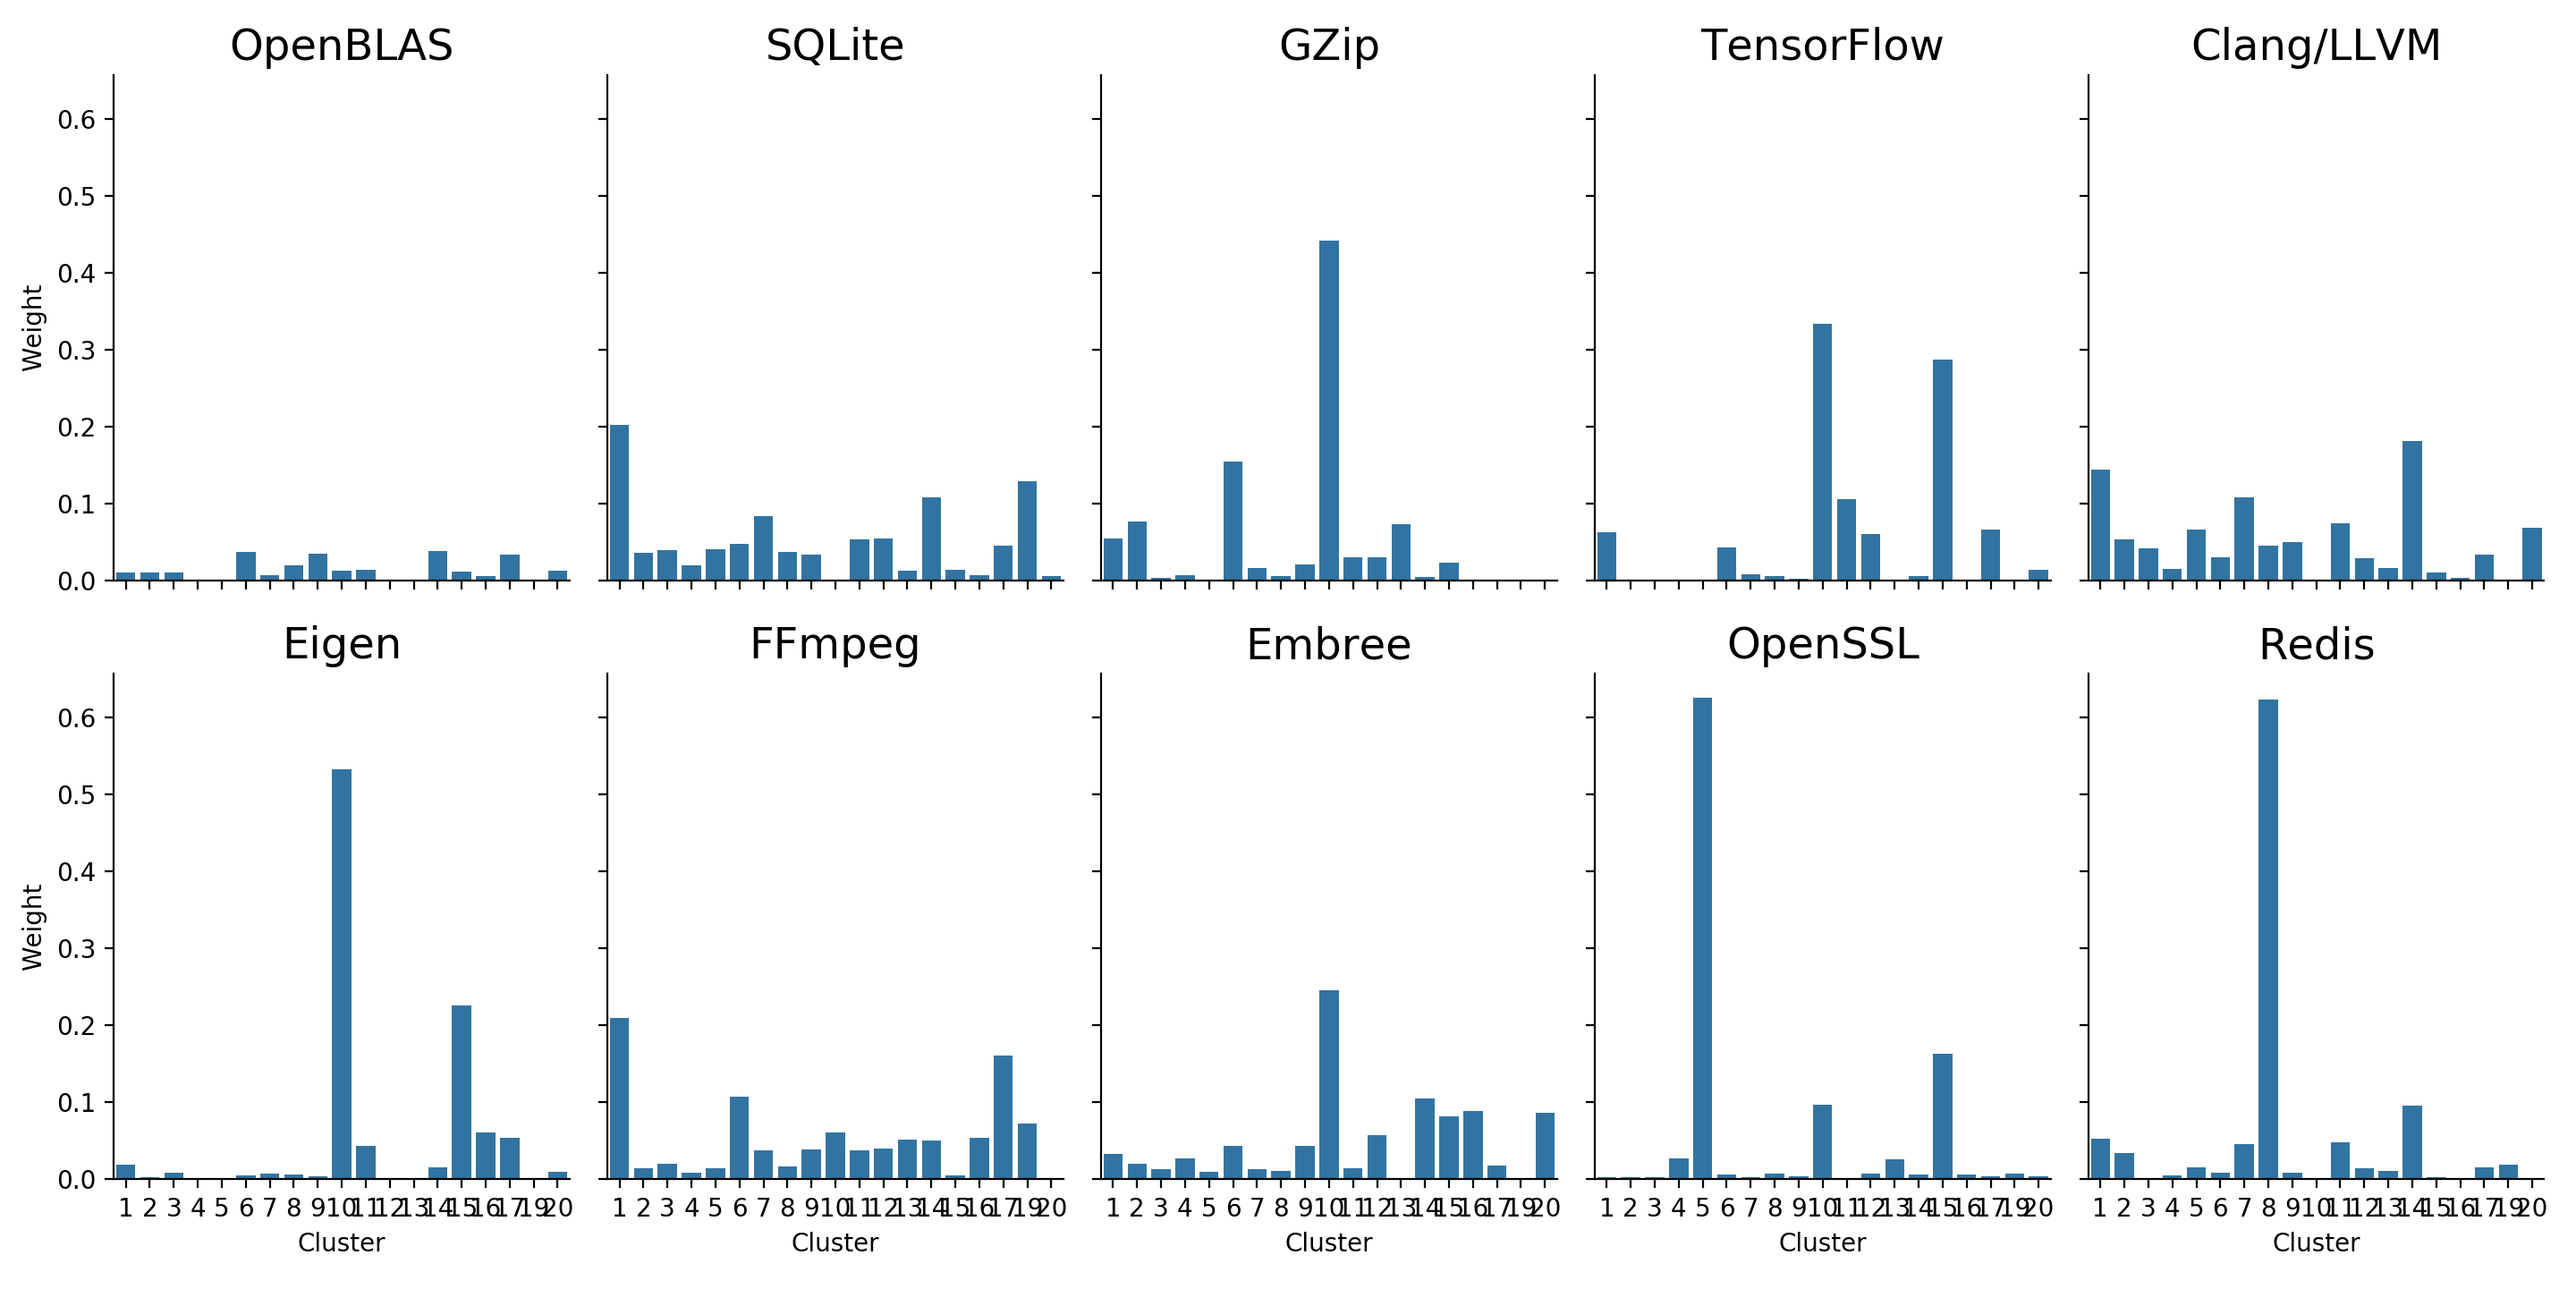
\includegraphics[width=\textwidth]{figures/apps-vs-clusters.png}
\caption{Breakdown of applications by basic block classes.
Y-axis represents the total weight of basic blocks
in a given class.
Cluster-16 contains vectorized basic blocks.
Note that the breakdown of OpenBLAS can be surprising
because the official benchmark contains
unoptimized verification code that got included into
our analysis}
\label{fig:apps_vs_clusters}
\end{figure*}

\section{Results}

\subsection{Evaluation of Existing Models}
We evaluated IACA, llvm-mca, Ithemal\cite{ithemal}, and OSACA\cite{osaca}
on three recent Intel microarchitectures: Ivy Bridge, Haswell, Skylake.
Some basic blocks in our dataset contains AVX2 instructions, which are not supported in Ivy Bridge,
and these basic blocks are not included in validation for Ivy Bridge.
We use relative error (i.e. absolute error of the predicted throughput normalized by the measured throughput)
as the metric to measure inaccuracy.
Table \ref{tab:overall} shows the unweighted average error
of each model on different microarchitectures.
% include ivb and skl
Figures \ref{fig:ivb-app-err}, \ref{fig:hsw-app-err}, and \ref{fig:skl-app-err}
show the breakdown of the errors by applications.
Figure \ref{fig:ivb-cluster-err}, \ref{fig:hsw-cluster-err}, 
and \ref{fig:skl-cluster-err} show the breakdown of the errors by basic block categories 
(see \ref{classification} for details of basic blocks classification).
We note that the overall error of each model can be unrepresentative
of its performance on a given domain.
The discrepancy between these models' overall unweighted accuracy
and that of specialized domains (e.g. numerical kernels) highlights
the need of basic block classification and per-class error reporting.

Generally speaking, basic blocks dominated by stores
(category-4) are easier to predict,
while the throughput of basic blocks that mixes load instructions
with other operations (e.g. category-8) are considerably
more difficult to predict -- the prediction error is on average more than
twice higher than predicting basic blocks with only stores. 
We surmise that this is due to weakness of existing analyzers to model 
memory dependence.
In addition to basic blocks with memory dependence,
vectorized basic blocks (e.g. category-2) also causes high prediction errors.

% TODO summarize error by applications

\textbf{IACA}~\cite{iaca} is relatively more stable compared to other models that we evaluated.
An interesting point to note is that IACA is consistently accurate on basic blocks from OpenSSL.

\textbf{llvm-mca} is on par with IACA on Ivy Bridge and Haswell but considerably worse on Skylake,
especially on modelling basic blocks involving basic arithmetic operations.
We suspect the decrease in performance in Skylake is a result of LLVM developers 
having less time updating the cost models for the relatively new microarchitecture.

\textbf{Ithemal}~\cite{ithemal} consistently outperforms other models, except on vectorized basic blocks (i.e. category-2).
Ithemal is also considerably better than other models at modelling basic blocks with memory dependence,
as demonstrated by its errors on predicting basic blocks from categories 4 and 8.
We discussed ithemal's underformance on vectorized basic blocks with the authors of Ithemal, who suggested that the inconsistency
was a result of imbalance in their training dataset;
the majority of which, similar to our data set, consists of non-vectorized basic blocks.
In addition, the authors of Ithemal reported having to leave more basic blocks out of the training of their
Skylake model due to lack of reliable throughput measurements.
% TODO comapre error to basic block length and show ithemal does not generalize to large baisc blocks

\textbf{OSACA}\cite{osaca} generally has higher errors compared to other models.
We note that this might have less to do with OSACA's methodology than the engineering of its instruction parser.
During our evaluations, we found and reported five bugs related to OSACA's instruction parser.
In particular, OSACA does not recognize several instruction forms;
depends on the cases, it either crashes or treats unrecognized instruction forms as nops.
One such instruction form is any instruction that reads an immediate operand and writes to memory
(e.g. \verb|add [rbx], 1|), and OSACA treats these instructions as nops, thus under-reporting the throughput of
many basic blocks.


\begin{table}
\begin{tabular}{|p{0.25\columnwidth}|p{0.3\columnwidth}|p{0.25\columnwidth}|}
\hline

Microarchitecture & Model & Average Error\\
\hline

Ivy Bridge & IACA & 0.1693\\
    & llvm-mca & 0.1885\\
    & Ithemal & 0.1180\\
    & OSACA & 0.3277\\
\hline

Haswell & IACA & 0.1798\\
    & llvm-mca & 0.1832\\
    & Ithemal & 0.1253\\
    & OSACA & 0.3916\\
    
\hline 
Skylake & IACA & 0.1578\\
    & llvm-mca & 0.2278\\
    & Ithemal & 0.1191\\
    & OSACA & 0.3768\\

\hline
% TODO more for IVB and SKL
\end{tabular}
\\
\caption{Overall error of evaluated models.}
\label{tab:overall}
\end{table}

\begin{figure}
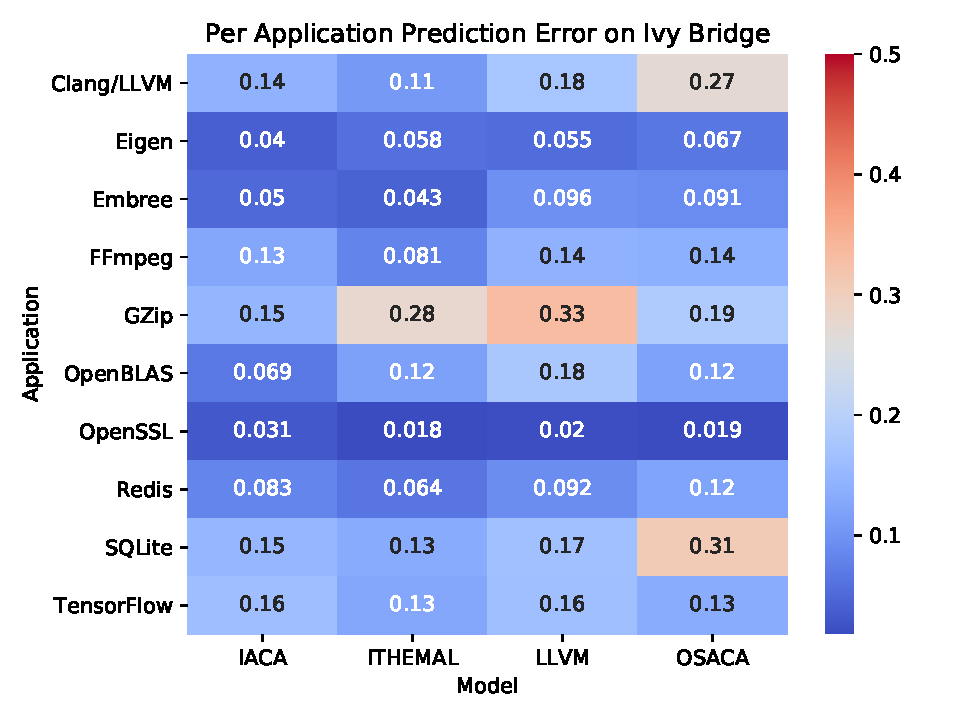
\includegraphics[width=\columnwidth]{figures/ivb-app-err.pdf}
\caption{Per-application error for each model on Ivy Bridge;
error for each basic block is weighted by the frequency it is sampled during profiling.}
\label{fig:ivb-app-err}
\end{figure}

\begin{figure}
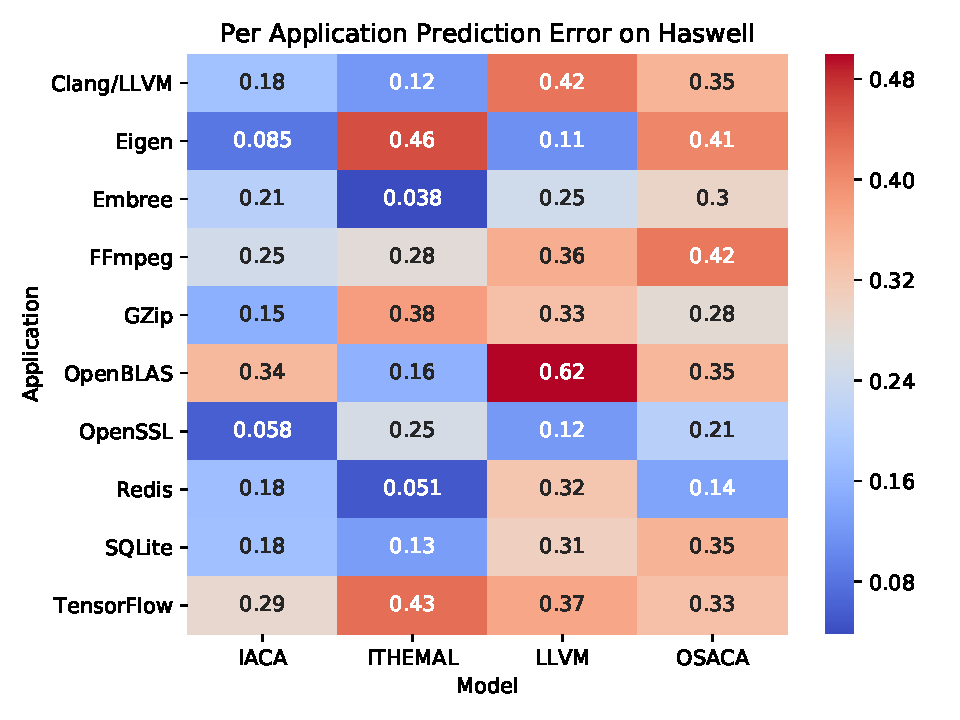
\includegraphics[width=\columnwidth]{figures/hsw-app-err.pdf}
\caption{Per-application error for each model on Haswell}
\label{fig:hsw-app-err}
\end{figure}

\begin{figure}
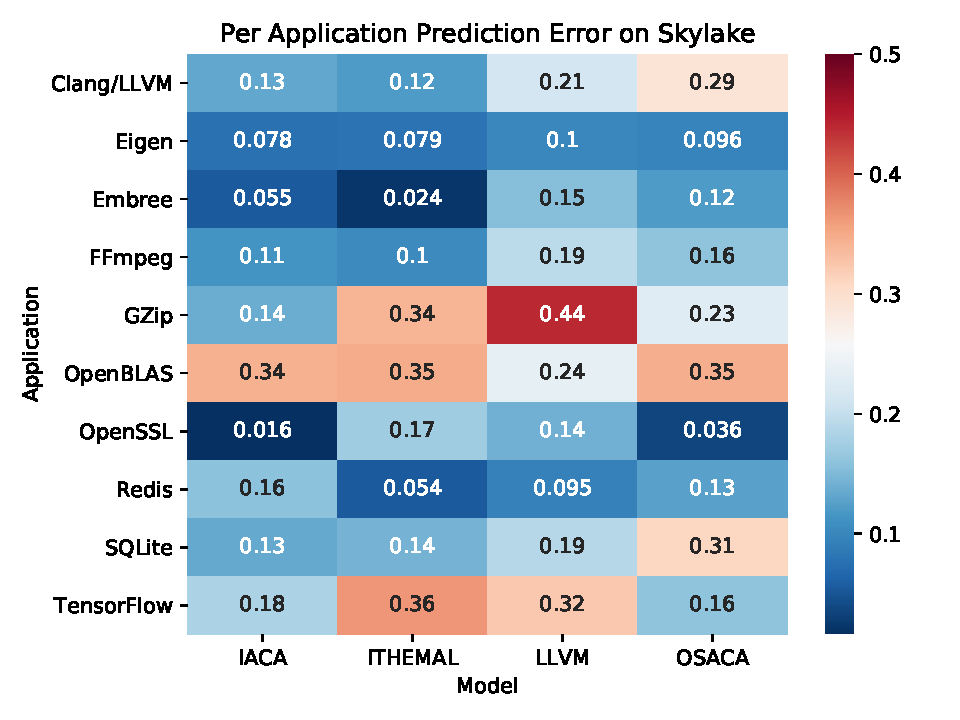
\includegraphics[width=\columnwidth]{figures/skl-app-err.pdf}
\caption{Per-application error for each model on Skylake. }
\label{fig:skl-app-err}
\end{figure}

\begin{figure}
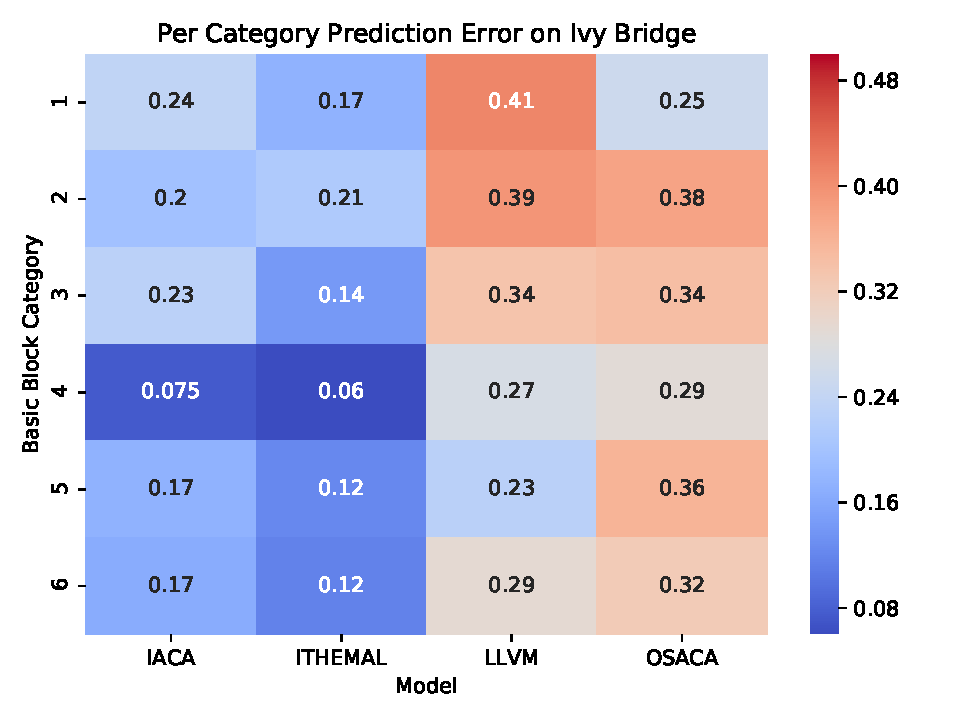
\includegraphics[width=\columnwidth]{figures/ivb-cluster-err.pdf}
\caption{Per-cluster error for each model on Ivy Bridge}
\label{fig:ivb-cluster-err}
\end{figure}

\begin{figure}
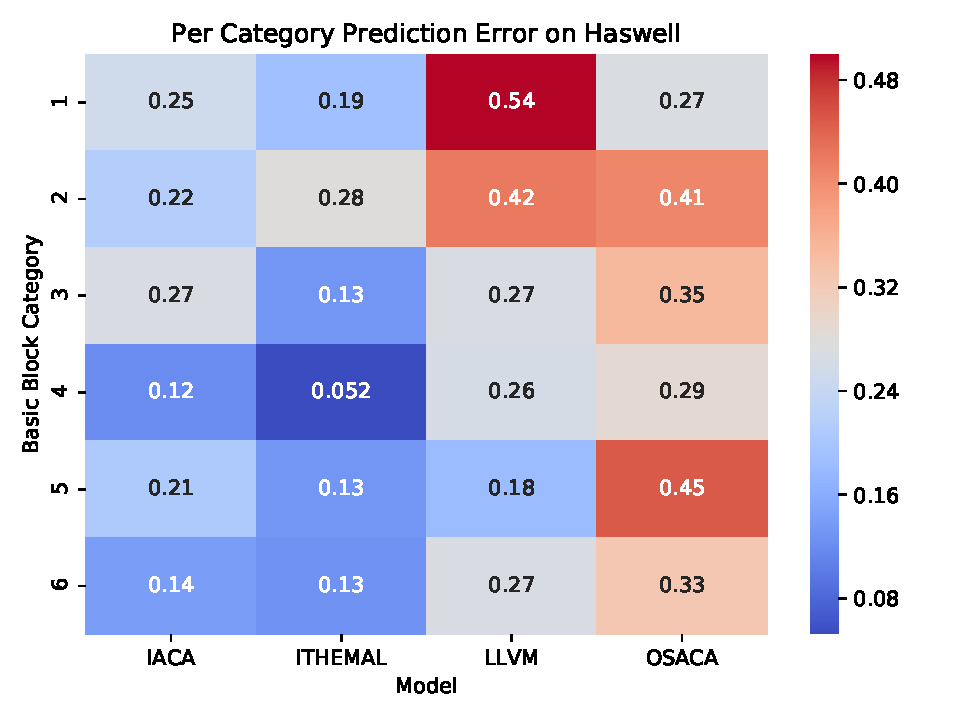
\includegraphics[width=\columnwidth]{figures/hsw-cluster-err.pdf}
\caption{Per-cluster error for each model on Haswell}
\label{fig:hsw-cluster-err}
\end{figure}

\begin{figure}
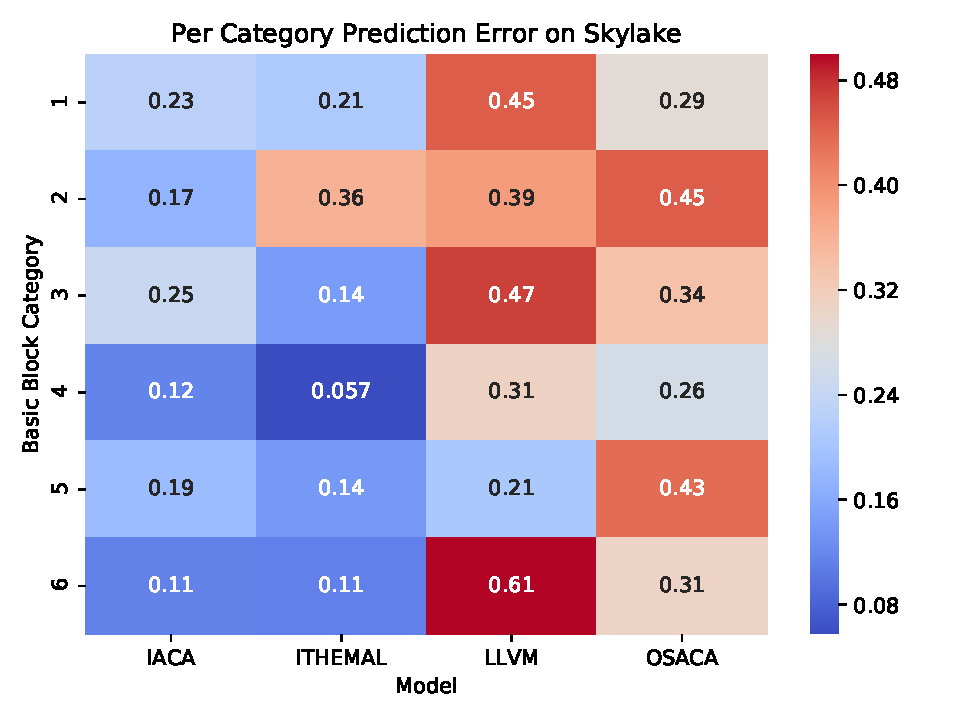
\includegraphics[width=\columnwidth]{figures/skl-cluster-err.pdf}
\caption{Per-cluster error for each model on Skylake}
\label{fig:skl-cluster-err}
\end{figure} 


\bibliographystyle{ieeetr}
\bibliography{paper}

\vspace{12pt}

\end{document}
